\section{Model Dynamics}
\label{sec:og.dynamics}

We are interested in the dynamics that emerge when fixing the parameters $\beta = 1, f = 150, L = 4.2 \cdot 10^{-3}, R = 2, V_m = 5,$ and $\mu = 0.5$.
The parameters $E_0$ and $\chi_0$ are varied.
$E_0$ is in the range $[14, 28]$, while $\chi_0$ is in the range $[0.1, 0.65]$.
When scanning this parameter plane for the period of stable cycles, \Cref{fig:yunus.2pi.2d.full} emerges.

\begin{figure}
    \centering
    \includegraphics[width=0.6\textwidth]{99_Yunus/2D_Period_Zoomed/result.png}
    \caption{2D Scan of Original Model}
    \label{fig:yunus.2pi.2d.full}
\end{figure}

The regions in \Cref{fig:yunus.2pi.2d.full} with the same color mean, that the stable cycles in these regions have the same period.
Points $A, B$ and $C$ are in the parameter region, which has stable cycles with the period 12.
The period regions, in which these points are, differ in another way.
Besides the period of a cycle, there is another characteristic, the symbolic sequence.
It describes, on which branches the points of the cycle exist.
Some cobwebs illustrate the difference between the parameter regions.
\Cref{fig:yunus.2pi.CobwebA12,fig:yunus.2pi.CobwebC12} how the cobwebs at points $A$ and $C$.
Both parameter regions have only one stable cycle of period 12.
The stable cycle at point $A$ has the symbolic sequence $\A^3\B^3\C^3\D^3$ and the cycle at point $C$ has the symbolic sequence $\A^2\B^4\C^2\D^4$.
\todo{better formulation for next sentence}
Where the first branch completely in the picture is denoted $\A$.
We say that such parameter regions are of ``type A'', while the parameter region for point $B$ is of ``type B''.

\Cref{fig:yunus.2pi.CobwebB12} shows the cobweb at point $B$.
We see directly that there are now two coexisting cycles of period 12.
One cycle has the symbolic sequence $\A^3\B^3\C^2\D^4$, while the other one has the symbolic sequence $\A^2\B^2\C^3\D^3$
We say that both of these are symmetric via rotation by $\pi$, meaning the two halves of the cycles are swapped.
These cycles behave similarly to both the cycles at points $A$ and $B$ in the following way.
The cycle $\Cycle{\A^3\B^3\C^2\D^4}$ behaves like the cycle $\Cycle{\A^3\B^3\C^3\D^3}$ at point $A$ on its left half, while it behaves like the cycle $\Cycle{\A^2\B^4\C^2\D^4}$ on its right half.
The same is true for the cycle $\Cycle{\A^2\B^4\C^3\D^3}$ but reversed since it is the other cycle rotated by $\pi$.

\begin{figure}
    \centering
    \begin{subfigure}{0.3\textwidth}
        \centering
        \includegraphics[width=\textwidth]{99_Yunus/Period12/Cobweb_A_12/result.png}
        \caption{At Point $A$}
        \label{fig:yunus.2pi.CobwebA12}
    \end{subfigure}
    \begin{subfigure}{0.3\textwidth}
        \centering
        \includegraphics[width=\textwidth]{99_Yunus/Period12/Cobweb_B_12/result.png}
        \caption{At Point $B$}
        \label{fig:yunus.2pi.CobwebB12}
    \end{subfigure}
    \begin{subfigure}{0.3\textwidth}
        \centering
        \includegraphics[width=\textwidth]{99_Yunus/Period12/Cobweb_C_12/result.png}
        \caption{At Point $C$}
        \label{fig:yunus.2pi.CobwebC12}
    \end{subfigure}
    \caption{Cobwebs of Full Original Model}
\end{figure}

On our journey, this will be our criteria for finding a minimal model reproducing these bifurcation phenomena.
We want a parameter region of ``type B'' next to two parameter regions of ``type A'', ideally in a chain.
Also the cycles in the parameter region of ``type B'' should behave like the stable cycles in the adjacent ``type A'' parameter regions on either half, like we just observed in the original model.
